\documentclass[11pt,a4paper]{article}
\usepackage[spanish,es-nodecimaldot]{babel}	% Utilizar español
\usepackage[utf8]{inputenc}					% Caracteres UTF-8
\usepackage{graphicx}						% Imagenes
\usepackage[hidelinks]{hyperref}			% Poner enlaces sin marcarlos en rojo
\usepackage{fancyhdr}						% Modificar encabezados y pies de pagina
\usepackage{float}							% Insertar figuras
\usepackage[textwidth=390pt]{geometry}		% Anchura de la pagina
\usepackage[nottoc]{tocbibind}				% Referencias (no incluir num pagina indice en Indice)
\usepackage{enumitem}						% Permitir enumerate con distintos simbolos
\usepackage[T1]{fontenc}					% Usar textsc en sections
\usepackage{amsmath}						% Símbolos matemáticos

% Comando para poner el nombre de la asignatura
\newcommand{\asignatura}{Programación Técnica y Científica}
\newcommand{\autor}{Vladislav Nikolov Vasilev}
\newcommand{\titulo}{Práctica 2}
\newcommand{\subtitulo}{Robótica}

% Configuracion de encabezados y pies de pagina
\pagestyle{fancy}
\lhead{\autor{}}
\rhead{\asignatura{}}
\lfoot{Grado en Ingeniería Informática}
\cfoot{}
\rfoot{\thepage}
\renewcommand{\headrulewidth}{0.4pt}		% Linea cabeza de pagina
\renewcommand{\footrulewidth}{0.4pt}		% Linea pie de pagina

\begin{document}
\pagenumbering{gobble}

% Pagina de titulo
\begin{titlepage}

\begin{minipage}{\textwidth}

\centering

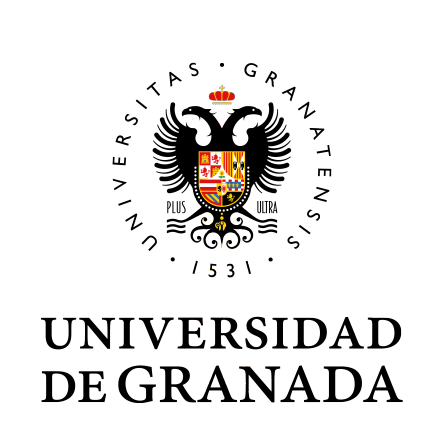
\includegraphics[scale=0.5]{img/ugr.png}\\

\textsc{\Large \asignatura{}\\[0.2cm]}
\textsc{GRADO EN INGENIERÍA INFORMÁTICA}\\[1cm]

\noindent\rule[-1ex]{\textwidth}{1pt}\\[1.5ex]
\textsc{{\Huge \titulo\\[0.5ex]}}
\textsc{{\Large \subtitulo\\}}
\noindent\rule[-1ex]{\textwidth}{2pt}\\[3.5ex]

\end{minipage}

\vspace{0.5cm}

\begin{minipage}{\textwidth}

\centering

\textbf{Autor}\\ {\autor{}}\\[2.5ex]
\textbf{Rama}\\ {Computación y Sistemas Inteligentes}\\[2.5ex]
\vspace{0.3cm}


\includegraphics[scale=0.3]{img/etsiit.jpeg}

\vspace{0.7cm}
\textsc{Escuela Técnica Superior de Ingenierías Informática y de Telecomunicación}\\
\vspace{1cm}
\textsc{Curso 2019-2020}
\end{minipage}
\end{titlepage}

\pagenumbering{arabic}
\tableofcontents
\thispagestyle{empty}				% No usar estilo en la pagina de indice

\newpage

\setlength{\parskip}{1em}

\section{Objetivo de la práctica}

El principal objetivo de esta práctica es hacer que un robot sea capaz de diferenciar
las piernas de las personas de objetos que no son piernas, como podrían ser por
ejemplo cilindros. Para ello, se ha propuesto utilizar un simulador donde se dispondrá
de un robot con un sensor láser y una cámara. Se tomarán primeramente datos y después
de procesarlos se entrenará un modelo de \textit{machine learning} que clasifique la
información como ``pierna'' y ``no pierna''. El modelo que se propone utilizar es un
\texttt{SVM}, y hay que escoger la mejor variante de dicho modelo comparando una serie
de \textit{kernels} e hiperparámetros. Una vez que se tenga el modelo definitivo, se utilizará
una escena de test para ver qué tan bien lo hace con datos nuevos. Finalmente se creará
un archivo en formato \texttt{HTML} que contendrá una tabla donde se mostrarán fotos de los
objetos detectados, además de la distancia a la que están del robot y de la clase real y
de la predicha.

En esta memoria se expondrá que \textit{scripts} se han utilizado, qué funcionalidad tiene cada
uno y se describirá brevemente lo que se ha ido haciendo.

\section{Captura de los datos}

Lo primero que se ha hecho ha sido capturar los datos. Para hacerlo, se ha creado un
\textit{script} llamado \textbf{capturar.py}, cuyo funcionamiento puede resumirse en
que pide al usuario el nombre del archivo de salida, el directorio donde quiere que
se guarde el fichero, el número de ciclos que se quiera leer y cuánto tiempo se tiene
que esperar entre lectura y lectura. Una vez hecho esto, se establece conexión
con el servidor de V-REP activo y se crea el directorio de salida y se cambia
el entorno de trabajo a este directorio. Una vez hecho esto, se toman los datos durante
tantos ciclos como se ha especificado anteriormente, haciendo una pausa entre cada captura
en la cantidad de segundos especificada. En cada lectura se van guardando los datos en el
fichero de salida. Además, se toma una captura de la cámara en la primera y en la última toma
de datos. Finalmente, se finaliza la conexión.

Para modularizar el código, el \textit{script} se ha estructurado en funciones. Estas
funciones se describen a continuación:

\begin{itemize}[label=\textbullet]
	\item \texttt{establecer\_conexion}: Establece la conexión con el servidor
	de V-REP activo y devuelve un ID del cliente. En caso de que no se pueda conectar,
	se finaliza la ejecución del \textit{script}.
	\item \texttt{obtener\_camara\_handler}: Obtiene un \textit{handler} de la cámara
	e inicializa la cámara y el sensor láser. Devuelve la referencia al \textit{handler}
	de la cámara para usos futuros.
	\item \texttt{init\_entorno}: Combina las dos funciones anteriores en una y devuelve
	tanto el ID del cliente como el \textit{handler} de la cámara.
	\item \texttt{procesar\_ciclo}: Esta función hace una captura del sensor laser y obtiene
	información sobre los puntos detectados en los ejes $X$ e $Y$. Una vez hecho esto, crea
	un diccionario que contiene información sobre la iteración actual y los puntos detectados
	en los dos ejes anteriores, con el mismo formato que el que se puede ver en los ficheros
	de ejemplo.
	\item \texttt{capturar\_guardar\_imagen}: Esta función hace una captura de lo que ve la
	cámara de la misma forma que se hacía en el código de ejemplo. Guarda el resultado
	en un fichero con un nombre específico.
	\item \texttt{stop\_simulacion\_conexion}: Con esta función se detiene la simulación
	que se está haciendo y se cierra la conexión con el servidor.
\end{itemize}

Para capturar los datos, se han creado 4 escenas: una con una persona de pie, una con una persona
sentada, una con un par de cilindros más pequeños que las piernas de una persona y otra
con un par de cilindros más grandes que las piernas de una persona. Para cada caso se han tomado
capturas de cerca, a distancia media y de lejos. Este proceso se puede ver a continuación:

\begin{figure}[H]
\centering
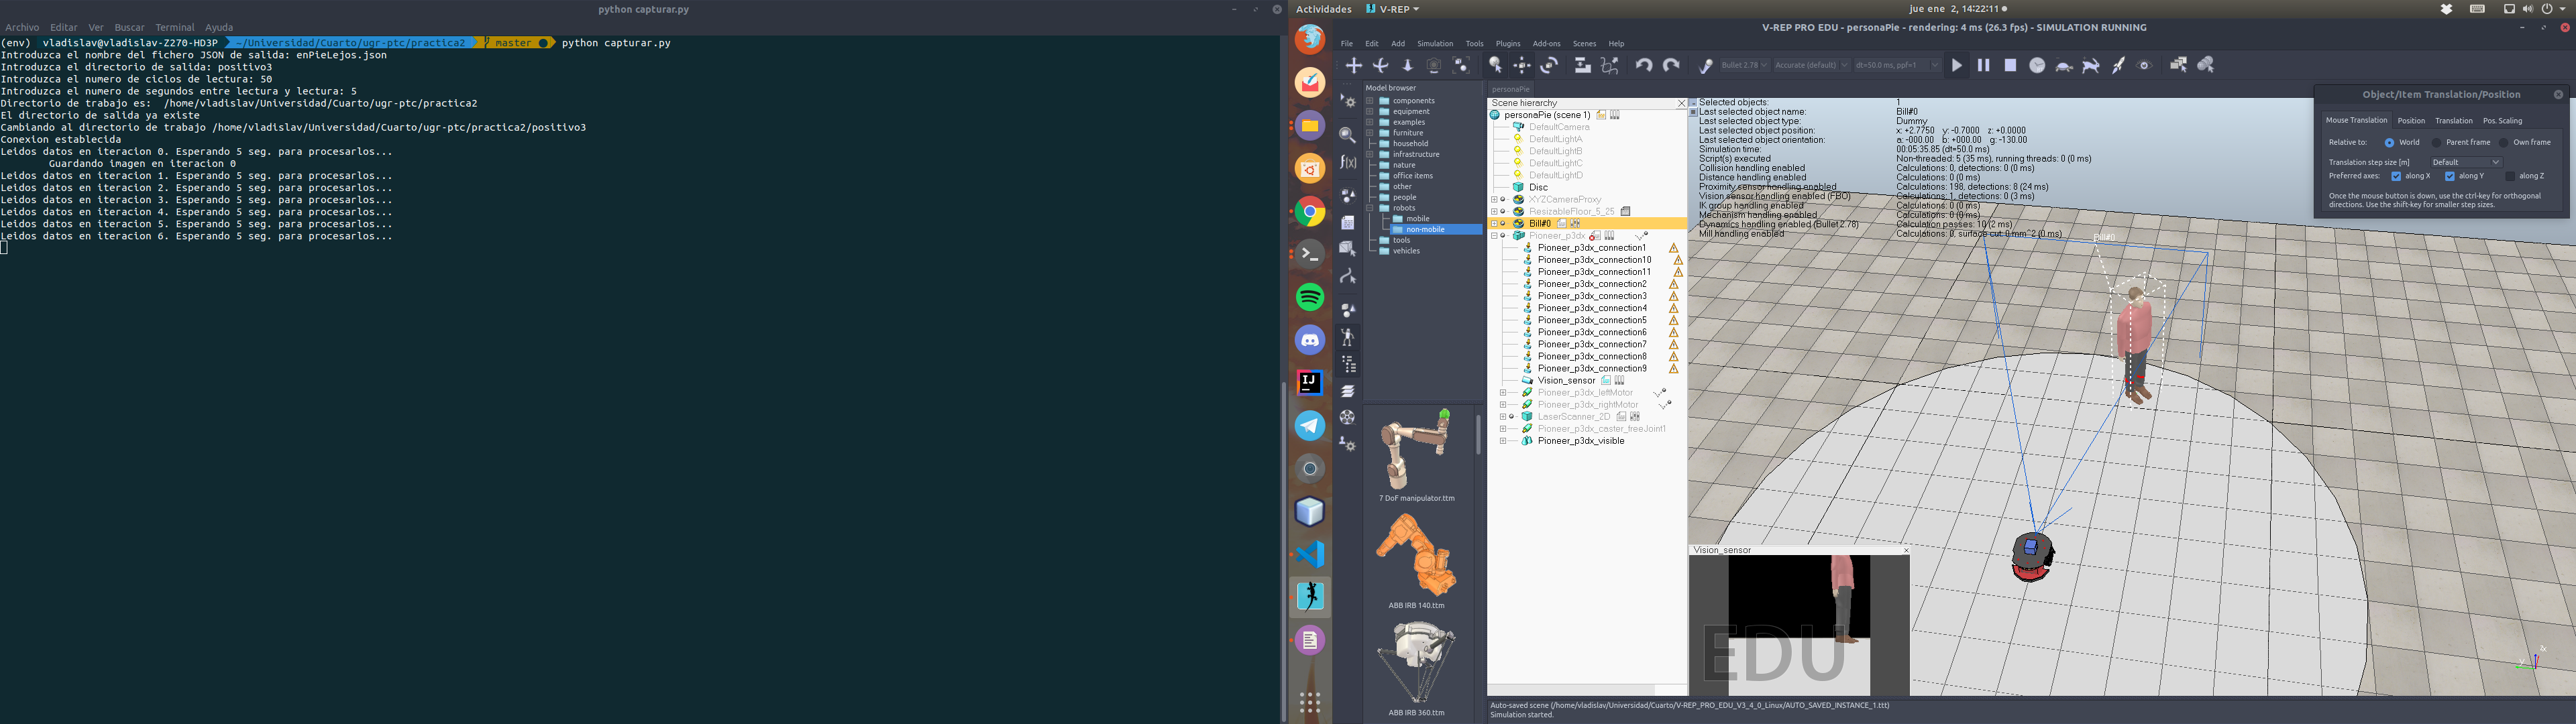
\includegraphics[scale=0.1]{img/pie2.png}
\caption{Captura de datos con persona de pie.}
\end{figure}

\begin{figure}[H]
\centering
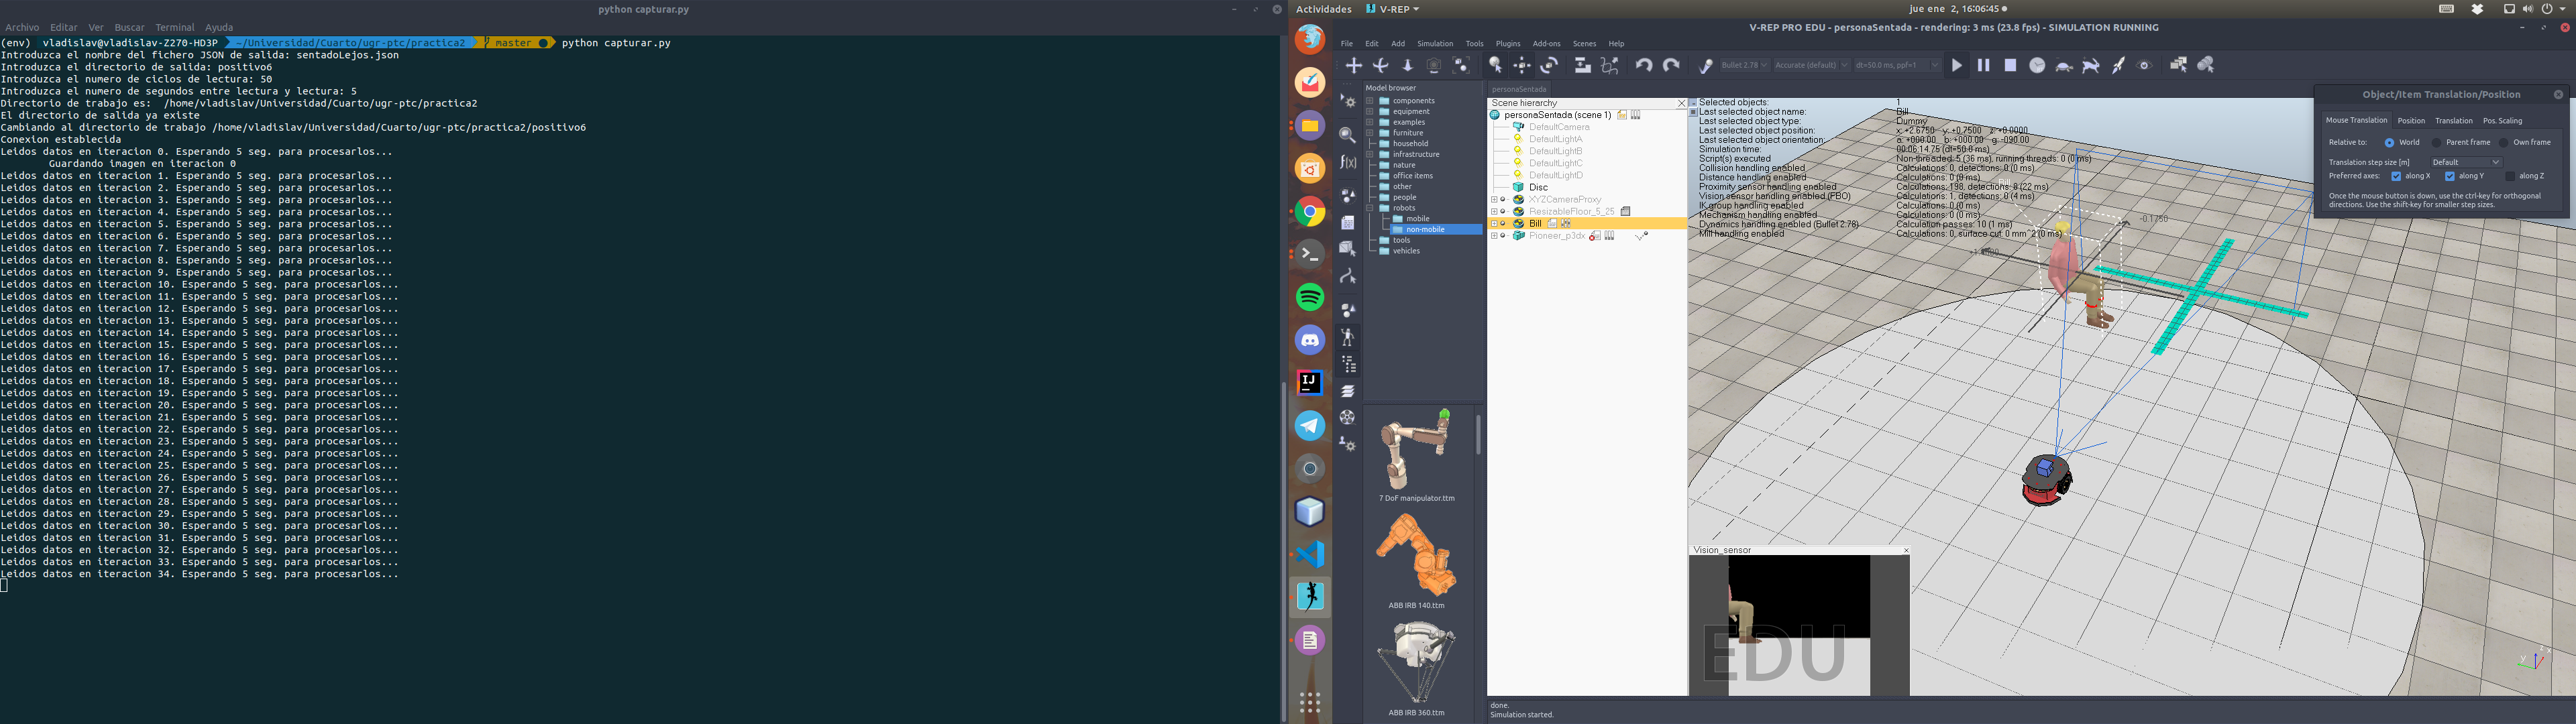
\includegraphics[scale=0.1]{img/sentado2.png}
\caption{Captura de datos con persona sentada.}
\end{figure}

\begin{figure}[H]
\centering
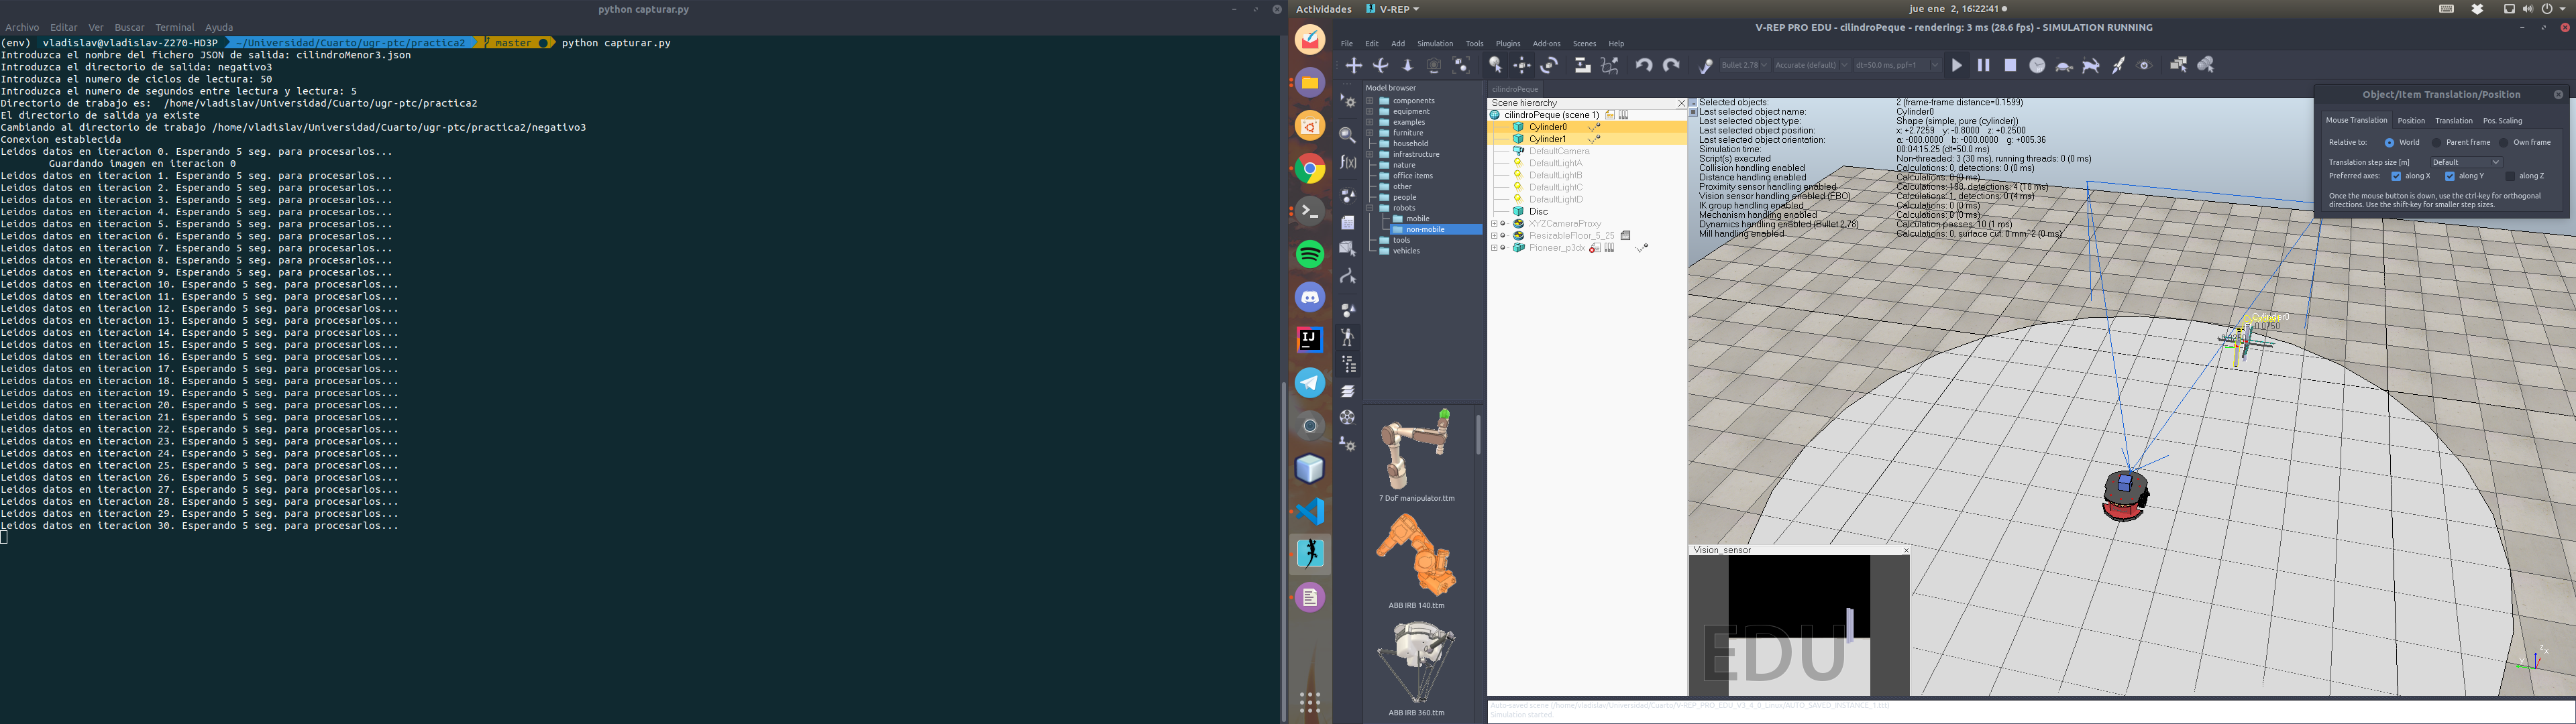
\includegraphics[scale=0.1]{img/peque2.png}
\caption{Captura de datos con par de cilindros pequeños.}
\end{figure}

\begin{figure}[H]
\centering
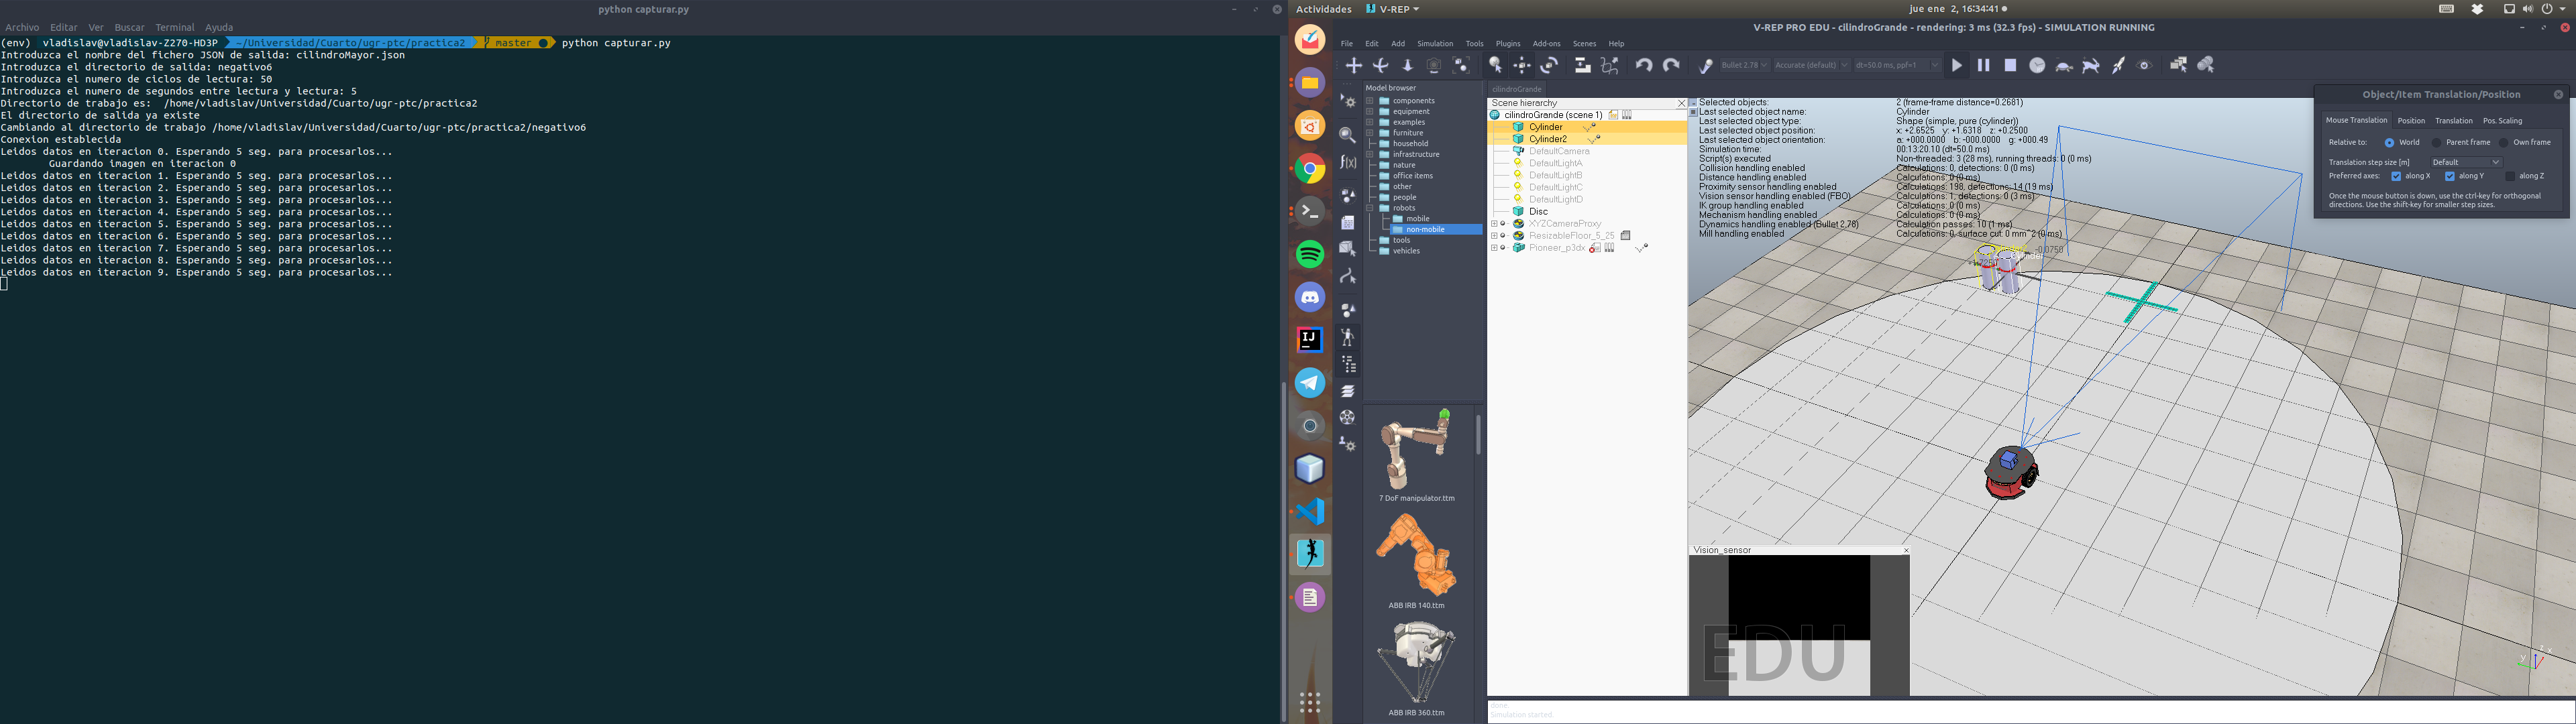
\includegraphics[scale=0.1]{img/grande2.png}
\caption{Captura de datos con par de cilindros grandes.}
\end{figure}

Como se puede ver, también se ha puesto un círculo en el suelo de radio $3.5$, el cuál sirve
de guía a la hora de tomar las capturas de los datos, para no salirse del radio especificado.

\section{Agrupación de los puntos en clusters}

Una vez que se han tomado los datos, hace falta agrupar los puntos en clusters. Para
ello se ha creado un \textit{script} llamado \textbf{agrupar.py} el cuál se encarga
precisamente de eso.

El funcionamiento general se resumen en que toma todos los directorios de ejemplos positivos
y de ejemplos negativos y crea clusters a partir de la información de cada tipo de directorio,
según el formato que se ha especificado.
Finalmente, guarda los ejemplos negativos en un fichero en formato \texttt{JSON} y los positivos
en otro, teniendo por tanto la información separada.

Para crear los clusters es necesario establecer el número mínimo de puntos que lo pueden formar,
el máximo y la distancia que puede haber, como máximo, entre dos puntos consecutivos.
En un primer instante había establecido que el \textbf{número mínimo de puntos} fuese 3,
el \textbf{número máximo de puntos} fuese 25 y la \textbf{distancia máxima entre dos puntos consecutivos}
fuese $0.03$. Sin embargo, estos valores se modificarán más adelante, aunque se comentará
en la sección correspondiente.

De nuevo, tal y como se hizo ante, se ha estructurado el fichero en funciones, las cuáles
se pueden ver a continuación:

\begin{itemize}[label=\textbullet]
	\item \texttt{obtener\_cluster\_datos}: Esta función se encarga de extraer un único
	cluster a partir de un conjunto de puntos. Recorre el \textit{array} de puntos
	proporcionado, el cuál está compuesto por coordenadas $(x, y)$, y va añadiendo
	los puntos consecutivos a una lista, siempre y cuando la distancia de un punto
	al siguiente no supere el umbral, haya menos puntos que el máximo permitido en la
	lista y no se supere la longitud del \textit{array} de entrada (ya que se está
	recorriendo con índices).
	\item \texttt{procesar\_clusters\_muestra}: Esta función procesa una muestra de datos,
	generando los clusters que se pueden encontrar en el conjunto de puntos. Utiliza la
	función anterior para determinar los clusters uno por uno y al final los
	junta en una única lista. Se acepta un cluster siempre y cuando el número de puntos
	supere al mínimo requerido. La función está pensada para que pueda recibir la inforamción
	como un diccionario de \texttt{Python}, de forma que se pueda reutilizar más adelante.
	Por tanto, si se le quiere pasar información que está en formato \texttt{JSON}, se tiene
	que cargar antes.
	\item \texttt{procesar\_clusters\_fichero}: Con esta función se pueden procesar
	los clusters de un fichero determinado. Hace uso de la función anterior, y junta
	los clusters de cada muestra en una única lista.
	\item \texttt{procesar\_clusters\_directorios}: Con esta función se pueden obtener
	los clusters de todos los archivos de un conjunto de directorios del mismo tipo.
	Para ello, se utiliza la función anterior, la cuál procesa cada fichero de forma
	individual. Se devuelve una lista con los clusters encontrados para todos los
	directorios del mismo tipo.
	\item \texttt{generar\_informacion\_cluster}: Esta función permite generar la información
	de salida de los clusters, en el formato especificado. Recibe la lista de clusters y construye
	una lista con diccionarios con el mismo formato.
	\item \texttt{guardar\_clusters}: Esta función permite guardar los clusters en un
	archivo con un nombre determinado. Para generar la información, utiliza la función
	anterior. Después, la transforma a formato \texttt{JSON} y la escribe en el fichero
	de salida.
\end{itemize}

\section{Extracción de características}

\section{Entrenamiento de un clasificador \texttt{SVM}}

\section{Predicción y corrección de los datos}

\section{Detección de objetos}

\end{document}

